%%%%%%%%%%%%%%%%%%%%%%%%%%%%%%%%%%%%%%%%%%%%%%%%%%%%%%%%%%%%
% Document settings
\documentclass{ACGSeminar}
\usepackage{tikz}
\usepackage{svg}
\usepackage{mathtools}

\tikzset{
  root/.style     = {draw=none},
  leaf/.style     = {draw=none},
  dummy/.style    = {circle,draw},
  text-node/.style    = {rectangle, rounded corners, align=center,draw},
}

\bibliography{references}

%%%%%%%%%%%%%%%%%%%%%%%%%%%%%
% Hyphenations here
%%%%%%%%%%%%%%%%%%%%%%%%%%%%%
\hyphenation{}

%%%%%%%%%%%%%%%%%%%%%%%%%%%%%
% Title, Author, etc.

\begin{document}

\title{Efficient Ray Tracing Techniques}

\author{Dario Seyb}

\maketitle

%%%%%%%%%%%%%%%%%%%%%%%%%%%%%%%%%%%%%%%%%%%%%%%%%%%%%%%%%%%%
% Abstract

\begin{abstract}%
Ray Tracing is next to rasterization the most widely used technique to generate discrete 2D images from continuous 3D scenes. Until recently ray tracing was too resource intensive to produce images in realtime, but advances in algorithms and hardware capabilities, most notably the introduction of GPGPU (General Purpose Graphics Processing Units), made near-realtime ray tracing feasible. In this report we will present some of the techniques which are used to achieve this.
\end{abstract}

\keywords{Ray Tracing, Acceleration Structures, Realtime Rendering, GPGPU}
\tableofcontents

%%%%%%%%%%%%%%%%%%%%%%%%%%%%%%%%%%%%%%%%%%%%%%%%%%%%%%%%%%%%
% Introduction

\section{Introduction}
The technique of tracing rays through a scene consisting of primitives and media has been known to the computational physics community for a long time. There it is mostly used to simulate the propagation of waves (e.g. shock waves of an earthquake) through a heterogeneous medium (e.g. the interior of the earth). \cite{GJI:GJI93}

It was first described in relation to computer graphics by Arthur Appel in 1968. At the time the common method to visualize three dimensional scenes was to synthesize two dimensional line and point drawings. Appel recognized the importance of shading and shadow casting in conveying shape and spatial relations. In his paper "Some techniques for shading machine renderings of solids" he proposes a method to realize this shading by casting rays originating from the viewers' position through each pixel on the viewing plane and calculating the first point of intersection with the scene. To determine shading he casts a second ray from this intersection point to the light source. Noteworthy is that he recognized Lambert's cosine law as the basis of a physically correct model for diffuse shading of surfaces lit by a point light.
\begin{equation}
I = S (Cosine L)/D^{2}
\end{equation}
Where $I$ is the final illumination intensity, $S$ the intensity of the light source, $L$ the angle between the surface normal and the direction to the light source and $D$ the distance to the light source.
Appel's technique was very compute intensive for its time, but already illustrated the power of ray tracing to generate realistic images using a relatively simple algorithm. \cite{Appel68}

\begin{figure}[htb!]
  \begin{centering}
    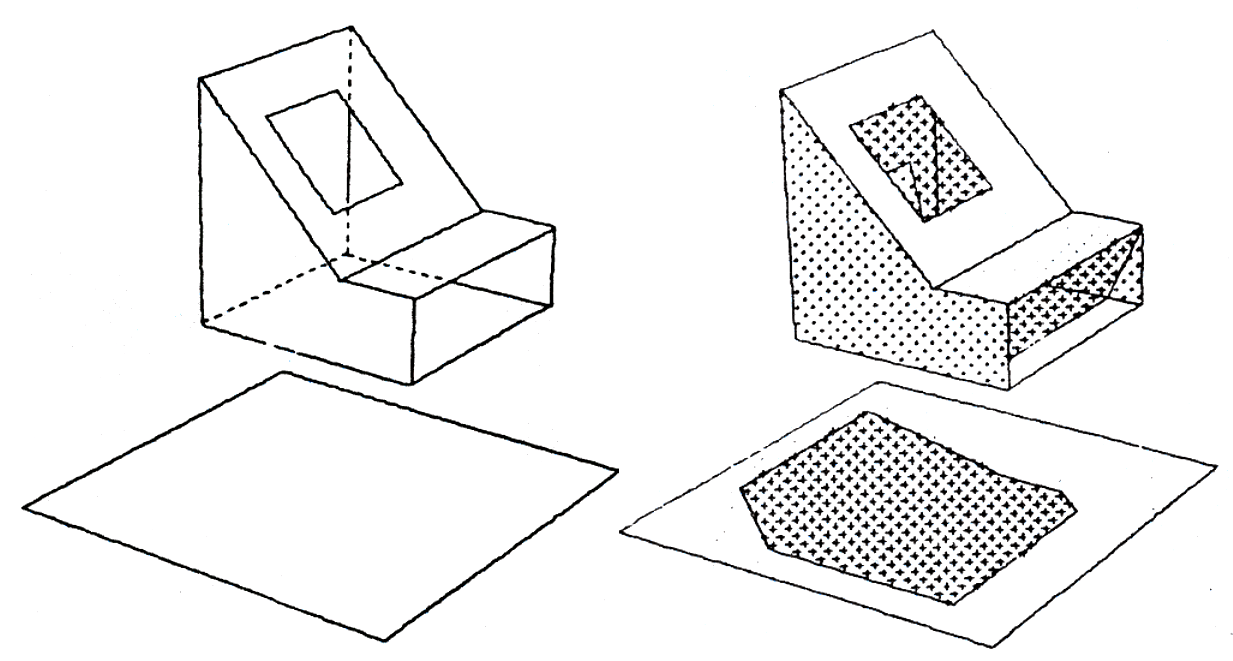
\includegraphics[width=10cm]{figures/Appel_Shading.png}\par
  \end{centering}
  \caption{Left: Unshaded Line/Point Drawing, Right: Drawing augmented with the technique introduced in \cite{Appel68}}
  \label{fig:appel_tracing}
\end{figure}

The next major contribution to ray tracing came from Turner Whitted of Bell Laboratories in 1980. In his landmark paper "An Improved Illumination Model for Shaded Display" \cite{Whitted:1980} he describes the algorithm that would become known as Recursive, or Whitted, Ray Tracing. So far ray tracing was only used to compute local illumination at the first point of intersection and the only secondary rays that were cast were shadow rays. This produced a fairly good approximation for diffuse surfaces, but was lacking in scenes with very reflective objects. Whitted took the concept of casting secondary rays and extended it to reflections and refractions. For each intersection point he proposed to not only compute a shadow ray in the direction of each light source, but also recursively compute the color of incoming reflected and refracted light. 
The model used to compute the illumination at a surface point is:

\begin{equation} \label{eq:illum-model}
I_{i}(x) = \overbrace{E_{i}(x)}^{\mathclap{\text{Emission}}} 
           + \underbrace{ k_{i}^{d} \sum_{j=1}^{n_{lights}} (N_{i}(x) \cdot L_{j})}_{\mathclap{\text{Direct/local illumination}}} 
           + \overbrace{k_{i}^{s}S_{i+1}(x)}^{\mathclap{\text{Specular lighting (reflected)}}} 
           + \underbrace{k_{i}^{t}T_{i+1}(x)}_{\mathclap{\text{Transmissive lighting (refracted)}}} 
\end{equation}

For each path through the scene like the one in Figure \ref{fig:ray-path} a tree of rays is build (see Figure \ref{fig:illum-tree}). This tree is evaluated bottom up using Equation \ref{eq:illum-model} and the value of the root node is stored as the pixel color.

\begin{figure}[htb!]
  \begin{centering}
    \includesvg[width=10cm]{out}\par
  \end{centering}
  \caption{Ray tree of path in Figure \ref{fig:ray-path}}
  \label{fig:ray-path}
\end{figure}

\begin{figure}[htb!]
  \begin{center}
  \begin{tikzpicture}
  [
    grow                    = down,
    sibling distance        = 6em,
    level distance          = 5em,
    edge from parent/.style = {draw, -latex},
    every node/.style       = {font=\footnotesize}
  ]
  \node [root] {}
    child { node [text-node] {$I_{0}$}
     child { node [text-node] {$I_{1}$}
        child { node [leaf] {...}
                edge from parent node [above left] {$T_{2}$} }
        child { node [leaf] {...}
                edge from parent node [above right] {$R_{2}$} }
        edge from parent node [above left] {$T_{1}$} }
     child { node [leaf] {...}
        edge from parent node [above right]{$R_{1}$} }
     edge from parent node [above left] {I} 
   };
  \end{tikzpicture}
  \end{center}
  \caption{Ray tree of path in Figure \ref{fig:ray-path}}
  \label{fig:illum-tree}
\end{figure}
This technique produced fairly realistic looking results, but Whitted himself acknowledged that it did not provide a solution to global illumination since objects could not act as light sources themselves and diffuse interreflections where not accounted for.

Over the next years many different approaches to solve this issue where proposed and in 1986 James T. Kajiya published a paper titled "The Rendering Equation"  \cite{Kajiya:1986} in which he presents an equation to describe the propagation of light in a scene. It is general enough to describe all optical phenomena we care about in computer graphics and this made it possible to classify rendering algorithms by how well they approximate a solution to the rendering equation.

\begin{equation} \label{eq:rendering-equation}
I(x,x')=g(x,x') [\epsilon(x,x') + \int_{S}{p(x,x',x'')I(x',x'')dx''}]
\end{equation}

The main difference between rendering algorithms is how they approach the evaluation of the integral in \eqref{eq:rendering-equation}. It cannot be evaluated analytically for scenes which are even remotely interesting, but the formulation of the rendering problem as an integral equation allows us to employ methods from calculus to devise new algorithms. This is where the idea of path tracing stems from.

%Finish Whitted, talk about recursiveness. Note his own comment about missing diffuse reflection
%Kajiya, rendering equation
%Talk about Veach and path tracing

%%%%%%%%%%%%%%%%%%%%%%%%%%%%%%%%%%%%%%%%%%%%%%%%%%%%%%%%%%%%
% Second Section
\section{Overview over the path tracing algorithm}
A short overview of the base algorithm we are going to use for the rest of the paper. Cite \cite{veach1997robust} all the way.

% Path integral formulation, monte carlo methods

\section{Spacial partitioning and acceleration structures}
Going logarithmic!
\subsection{BSP and KD-Trees}
\subsection{Volume Hierarchies}

\section{Reducing Variance}
Here's where \cite{Pharr:2010:PBR:1854996} comes in.
\subsection{Gradient-Domain Path Tracing}
Do I really want to go here? \cite{Kettunen2015sg} I'll implement everything else first and see if I have time left.
\subsection{Temporal Supersampling}
I need to find a real paper describing this, so far only GDC talks. I think this is going to make a huge difference in the quality I can achieve.

% Reference back to monte carlo, main issue of path tracing is variance expressed as noise, we need more samples. Temporal Supersampling provides these.

\section{Adapting the described algorithms to the GPU}
\subsection{Accessing the GPU outside of the rasterization pipeline}
Compute shaders
% Easier integration with OpenGL (needed for TXAA)
\subsection{Hierarchical data structures on the GPU}
Use this: \cite{Karras:2012:MPC:2383795.2383801}

\section{Results}
I plan to implement everything I describe since I strongly believe computer science papers should \textbf{always} come with code.
\subsection{Images}
Pretty images rendered in real time. Link to a video.
\subsection{Timings}
Timing comparisons between the different techniques.


\begin{figure}[htb!]
  \begin{centering}
    \includegraphics[width=10cm]{figures/Output_PT_10kSPP.png}\par
  \end{centering}
  \caption{This is what my path tracer is rendering right now, but not in real time.}
  \label{fig:pathtraced}
\end{figure}

%%%%%%%%%%%%%%%%%%%%%%%%%%%%%%%%%%%%%%%%%%%%%%%%%%%%%%%%%%%%
% Bibliography

\printbibliography
\cleardoublepage

\end{document}
